
\documentclass[12pt]{article}
\usepackage[margin=1in]{geometry}
\usepackage{times}
\usepackage{graphicx}
\usepackage{caption}
\usepackage{enumitem}
\usepackage{textgreek}

\date{}

\begin{document}

\title{\vspace{-3.0cm}\normalsize \textbf{Processing of Scalar Implicatures and Contextual Cues}}
       
\maketitle
\vspace{-2.8cm}

\paragraph{Introduction} 
While communicating, listeners infer what is implicated by the speaker by making use of various linguistic and contextual cues available to them. The scalar implicature in (1) can be interpreted semantically as "You got at least one gumball" and pragmatically with some's upper bound meaning as "You got some, but not all, of the gumballs". When the partitive 'of' is not used with 'some' as in (2), its absence provides a lexical cue to the listener and affects the strength of the implicature. Similarly, when the listener knows that this utterance is produced as a response to (3), they might be more or less likely to draw the implicature. 

\indent (1) You got some of the gumballs.\\
\indent (2) You got some gumballs.\\
\indent (3) Did I get all of the gumballs?

% \vspace{-\baselineskip} 
% To what extent does the contextual support provided by implicit QUD and a lexical cue (absence of partitive "of") modulate robustness and speed of scalar inferences? 

%Previous research suggests that .. alternatives, naturalness of alternatives etc

% Mention QUD before Experiments & relevanct QUD == allQUD (or stick to one)

\paragraph{Experiments} Both experiments investigated the robustness and speed of scalar inferences by using a 'gumball paradigm'. On each trial, participants saw a gumball machine with an upper chamber with 13 gumballs and an empty lower chamber. On critical trials, after 2 seconds, all 13 gumballs dropped to the lower chamber and participants heard the statement "You got some of the gumballs" (Experiment 1) or "You got some gumballs" (Experiment 2). At the beginning of both experiments, participants got assigned to one of the three groups (all-QUD, any-QUD, no-QUD) and were presented with a different cover story. These cover stories were designed to establish an implicit QUD. Participants in all-QUD group read that they are at a candy store helping a store worker test faulty gumball machines. The store owner threatened to fire the worker if the gumball machines are left empty and the worker can't see the machines. Participants were asked to help the store worker by telling him whether they agree or disagree with the statement.\\
\indent\textbf{all-QUD:} Is the machine empty? $\rightarrow$ Did I get all of the gumballs?\\
Participants in the any-QUD group read the same story except in their story, the store worker’s boss has threatened to fire him if the gumball machines get jammed.\\
\indent\textbf{any-QUD:} Is the machine jammed? $\rightarrow$ Did I get none of the gumballs?\\
Participants in no-QUD group didn't read a cover story but instead received instructions.\\
\indent\textbf{no-QUD:} Is the statement correct? $\rightarrow$ No implicit QUD 


\paragraph{Results} 
% \vspace{-\baselineskip} 
\paragraph{Judgements}
Absence of the partitive ’of’ lead to more semantic responses regardless of the implicit QUD and relevance of the QUD lead to more pragmatic responses regardless of the presence of the lexical cue. In both experiments, participants in the all-QUD group gave the most number of pragmatic responses and participants in the no-QUD groups gave the least.

A mixed effects logistic regression predicting response type with random by-participants intercepts from fixed effects of QUD found a main effect of QUD such that there are more pragmatic (NO) responses for all-QUD compared to any-QUD (Experiment 1: β=1.28, SE=0.52, p$>$0.0001, Experiment 2: β=3.81, SE=0.52, p$>$0.0001) and no-QUD (Experiment 1: β=2.07, SE=0.63, p$>$0.0001, Experiment 2: β=3.45, SE=0.58, p$>$0.0001).

\paragraph{Response Times}
Overall, the absence of the partitive lead to faster responses. When there was no implicit QUD and the partitive was present, pragmatic responses were faster than semantic ones, and when the simple some was used, semantic responses became faster than pragmatic ones.

The QUD affected the response time for semantic and pragmatic responses differently. The more relevant the alternative, the faster the pragmatic responses became and the slower the semantic responses became.
The two cues interacted in a way such that the absence of the partitive changed the faster response type in all QUD groups. The fastest responses were observed when 1) partitive was present, QUD was relevant and participants responded pragmatically and 2) partitive was absent, QUD was less relevant and participants responded semantically.
A mixed effects linear regression model with random by-participant in tercepts predicting log-transformed response time from fixed effects of QUD, response type and their interaction, revealed a main effect of response type such that NO responses were always faster than YES responses (β=1.28, SE=0.02, p$>$0.0001). The interaction between response type and QUD was also found to be significant such that in the all QUD group, NO responses were faster and YES responses were slower compared to any QUD group (β=- 0.11, SE=0.02, p$>$0.0001) and no QUD group (β=-0.07, SE=0.02, p$>$0.001). Response type was centered before entering the analysis.

\paragraph{Responder Type}
In the post hoc analysis, participants were divided into two groups as semantic and pragmatic responders. We investigated whether responder type affect speed of processing differently for different responder groups and whether this is affected by contextual cues. Semantic responders are participants who gave semantic responses more than half of the time ($>$4) and pragmatic responders are participants who gave pragmatic responses more than half of the time. Participants who gave the same number of pragmatic and semantic responses were excluded from this visualization and analysis.
In both experiments, and in each QUD group, pragmatic responders were faster to respond pragmatically and semantic responders were faster to respond semantically. The partitive didn’t affect the response times of different responders significantly. However, with increasing relevance of the QUD, pragmatic responders got faster at responding pragmatically and semantic responders got slower in responding semantically.

\pagebreak

\begin{figure}[!ht]  
    \begin{minipage}{.5\textwidth}
        \caption*{Experiment 1}
        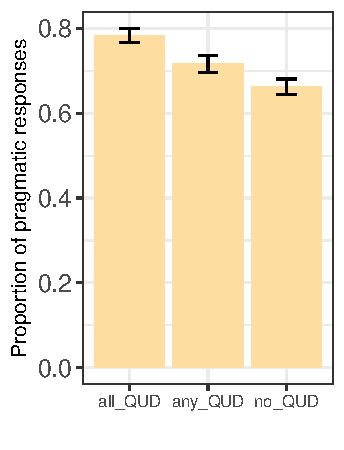
\includegraphics[height=9cm]{img/exp1_proportion_pragmatic.pdf}   
        \end{minipage}%
    \begin{minipage}{.5\textwidth}
        \caption*{Experiment 2}
        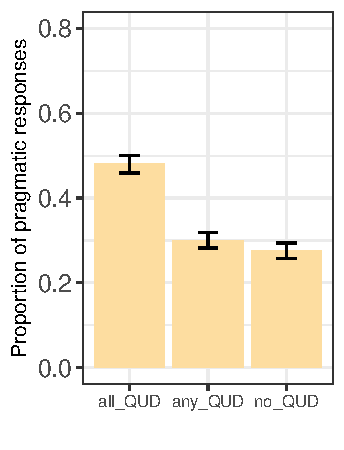
\includegraphics[height=9cm]{img/exp2_proportion_pragmatic.pdf}
        \end{minipage}%
        \caption{Proportion of pragmatic responses on critical trials}
    \end{figure}

\begin{figure}[!ht] 
    \begin{minipage}{.5\textwidth}
    \caption*{Experiment 1}
    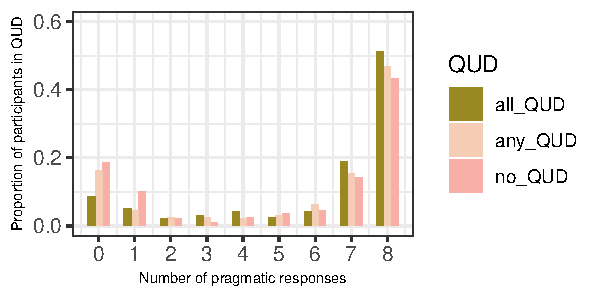
\includegraphics[height=5.6cm]{img/exp1_pragmatic_proportion.pdf}
    \end{minipage}%
    \begin{minipage}{.5\textwidth}
    \caption*{Experiment 2}
    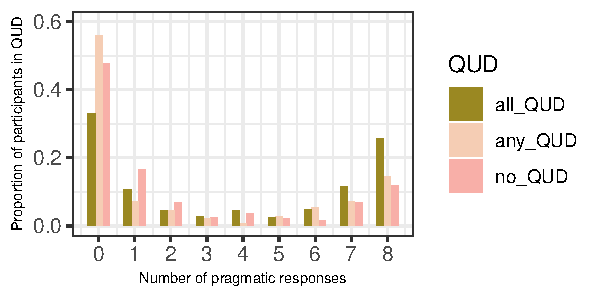
\includegraphics[height=5.6cm]{img/exp2_pragmatic_proportion.pdf}
    \end{minipage}%
    \caption{Distribution of participants over number of pragmatic responses on critical trials}
\end{figure}

\begin{figure}[!ht] 
    \begin{minipage}{.5\textwidth}
        \caption*{Experiment 1}
        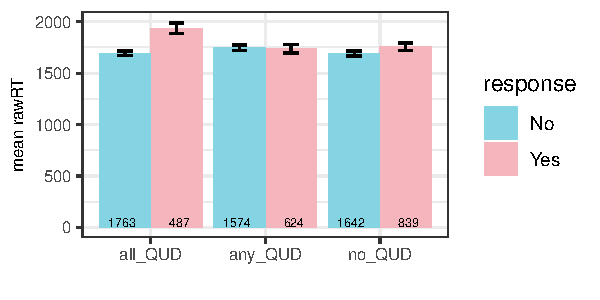
\includegraphics[height=5.2cm]{img/exp1_response_time.pdf}
    \end{minipage}%
    \begin{minipage}{.5\textwidth}
        \caption*{Experiment 2}
        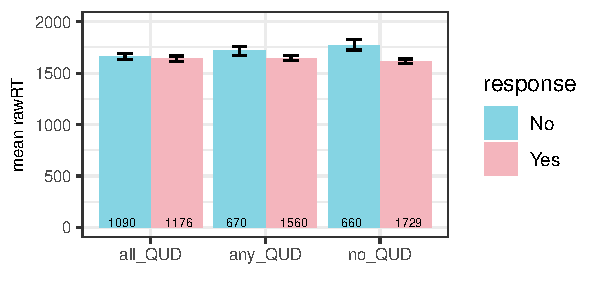
\includegraphics[height=5.2cm]{img/exp2_response_time.pdf}
    \end{minipage}%
    \caption{Mean response times for semantic and pragmatic responses on critical trials as a function of QUD}
\end{figure}

\begin{figure}[!ht] 
    \begin{minipage}{.5\textwidth}
        \caption*{Experiment 1}
        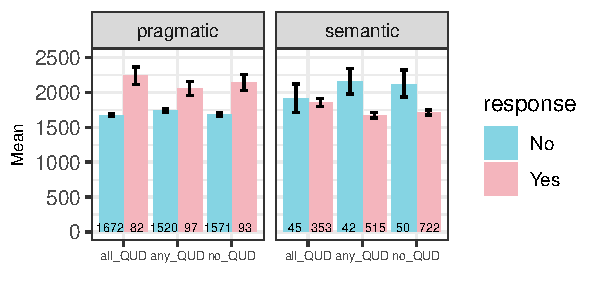
\includegraphics[height=5.4cm]{img/exp1_responder.pdf}
    \end{minipage}%
    \begin{minipage}{.5\textwidth}
        \caption*{Experiment 2}
        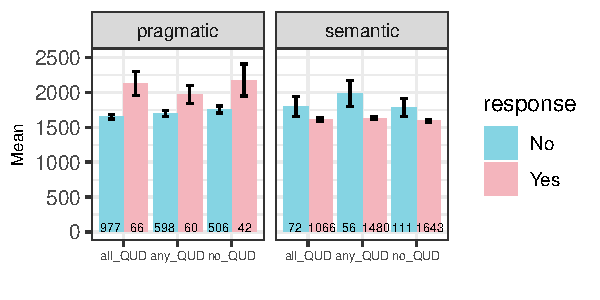
\includegraphics[height=5.4cm]{img/exp2_responder.pdf}
    \end{minipage}%
    \caption{Mean response times for semantic and pragmatic responders (inconsistent responders excluded)}
\end{figure}


\end{document}

% Previous research suggests that ...
% citations on role of context - alternatives, naturalness of alternatives
